\chapter{Partie électronique}

Dans cette partie, nous nous interréserons à la partie électronique de notre projet. Elle s'acompagnera d'explications théoriques sur les différents composants que nous utilisons sur notre réalisation.

\section{Une plateforme pour reçevoir les données}

Comme vu dans la partie précédente, notre projet consiste à capter, au départ, des données météorologiques. Pour faire cela, il nous faut un plateforme qui puisse communiquer avec des capteurs.

Naturellement, nous nous sommes tournés vers un \emph{Arduino}.

\subsection{Qu'est-qu'un Arduino ?}

Un Arduino est une plateforme possédant des entrées et des sorties. Il est organisé autour d'un microcontrôleur Atmel. Celui-ci est capable des contrôler différents récepteur comme une LED, un moteur ou encore un autre microcontrôleur. Il est capable également de recevoir et traiter des données d'un capteur. C'est dans ce cas que nous allons l'utiliser.

Les entrées et les sorties sont commandés à partie d'un code compilé sur un ordinateur puis téléversé sur un microcontrôleur.

Il existe une multitude de carte Arduino. Pour nos besoins, nous allons utiliser un \emph{Arduino Uno}. C'est une carte qui comporte 13 entrées/sorties numériques et 6 analogiques.

\begin{figure}[!h]
	\centering
	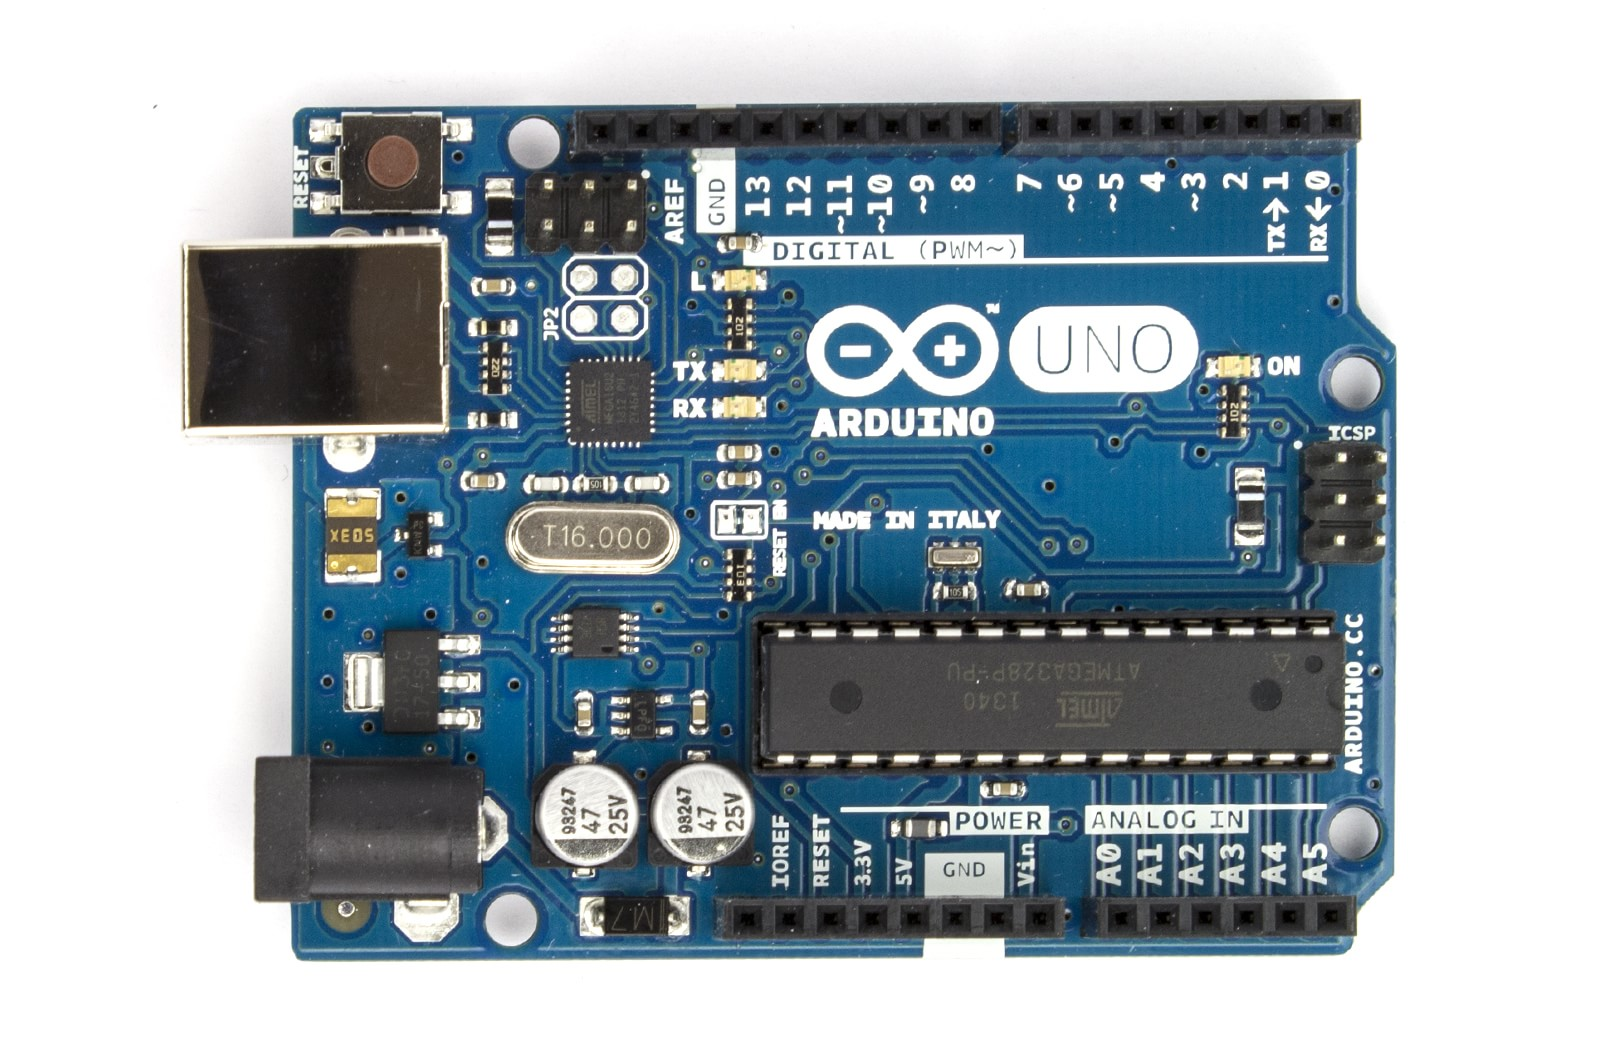
\includegraphics[width=.4\linewidth]{Images/Arduino_Uno}
	\caption{Un Arduino Uno R3}
\end{figure}

\subsection{Programmation d'un Arduino}

Pour programmer un Arduino, il faut utiliser un ordinateur avec l'IDE\footnote{Disponible sur \url{http://arduino.cc/en/Main/Software}.} du constructeur. Après l'avoir installé et configuré pour qu'il programme la bonne carte, nous pouvons y insérer du code.

La langage pour programmer un Arduino est très proche du C++, il s'agit en fait d'une surcouche. De ce fait, ce langage intègre la programmation orientée objet qui est très utile quand on veut développer : cela permet d'écrire du code plus compréhensible.

La structure d'un code Arduino se divise essentiellement en 2 parties : la première pour initialiser les différents composants, la seconde contient le code qui doit s'exécuter en boucle. Ainsi, pour faire clignoter une LED raccordée à la sortie 13, on peut téléverser le code suivant à l'Arduino.

\FichierCode{C++}{Codes/Exemple_Arduino.ino}

Comme vous pouvez le voir, le code est relativement simple. C'est pourquoi les plateformes Arduino sont conseillés pour les débutants (comme nous) en électronique. Dans ce code, il est possible d'ajouter des conditions avec \verb-if .. elseif ... else ...- ou des boucles \verb-for- ou \verb-while- pour faire des exemples plus complets.

\section{Le choix du capteur}

Afin de relever nos données météorologiques, il nous faut un capteur.

\subsection{Caractéristiques d'un capteur}

Un capteur est un composant permettant de traduire une grandeur physique en un courant électrique, hydrolique, \dots{} Les capteurs sont utilisés quasiment partout et il en existe beaucoup : certains peuvent capteur le courant, le vent, la température ou encore la lumière. Il s'agit en fait d'une interface entre le monde extérieur et un circuit électronique.

\paragraph{Type de sortie} Tout d'abord, il existe principalement deux types des capteurs qui se classent en fonction du leur sortie. Les capteurs analogiques sortent une tension ou une intensité qui se traduit par la valeur que capte ce composant.

Nous pouvons trouver également des capteurs numériques qui ne sortent pas un courant mais des états logiques : 0 ou 1. Nous allons nous tourner vers ce type de capteur

\paragraph{Caractéristiques} Pour distinguer différents capteurs, il existe des caractéristiques :
\begin{itemize}
	\item l'étendue : c'est l'écart entre la plus grande et la plus petit valeur mesurable,
	\item la résolution : c'est la plus petite variation que la capteur est capable de mesurées. Par exemple, un capteur de température capable de distinguer au maximum \SI{20,0}{\celsius} de \SI{20,1}{\celsius} à une résolution de \SI{0,1}{\celsius} ;
	\item la sensibilité : c'est la rapport entre la variation du signal d'entrée et la variation du signal du sortie ;
	\item l'exactitude : elle indique le pourcentage d'erreurs commises ;
	\item la justesse : c'est l'aptitude à donner un valeur juste, c'est l'écart entre le résultat moyen et la valeur vraie ;
	\item la fidélité : elle définit la dispersion des valeurs relevées.
\end{itemize}

En fonction de ces différentes caractéristiques, nous pouvons choisir un capteur.

\subsection{Capteur utilisé}

Comme vu dans le premier chapitre, notre capteur se doit de capter le température ainsi que la pression. Au lycée, nos deux professeurs nous ont orientées vers le capteur BMP180 en particulier celui de la marque Seeed Studio. Celui-ci a une particularité, il a besoin d'un \emph{shield} pour pouvoir être branché à un Arduino.

\begin{figure}
	\centering
	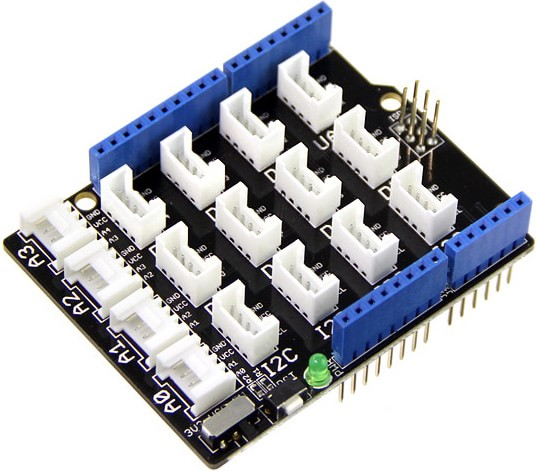
\includegraphics[width=.4\linewidth]{Images/Base_Shield}
	\hspace{.1\linewidth}
	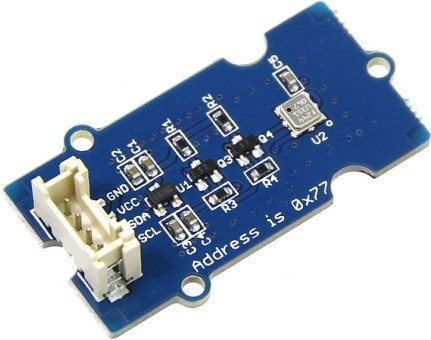
\includegraphics[width=.4\linewidth]{Images/BMP180}
	\caption{Le Base Shield V2 et le BMP180}
\end{figure}

Ce capteur se relie alors à une borne \verb-I2C- et le \emph{shield} se place sur l'Arduino. L'avantage de celui-ci est de permettre un cablage facile sans rajout de composants électroniques.

\subsubsection{Protocole I\up 2C}

Le capteur BMP180 se pilote à l'aide du protocole I\up 2C. Ce protocole est un bus série crée par Philips. Les échanges d'informations se font toujours entre un seul maître et un seul esclave (ici, l'Arduino et le capteur respectivement). La connexion des composants I\up 2C se fait par l'intermédiaire de trois fils :
\begin{itemize}
	\item la SDA (\emph{Serial Data Line}) : c'est la ligne de données ;
	\item la SCL (\emph{Serial Clock Line}) : c'est la ligne d'horloge ;
	\item la masse.
\end{itemize}
Pour un Arduino Uno, le fils pour la SDA doit se relier au \emph{pin} A4 et la SCL au \emph{pin} A5 mais cela nous est inutile grâce au \emph{shield}.

\subsubsection{Sa programmation}

Pour communiquer avec le capteur, il va falloir programmer l'Arduino. Pour cela, le constructeur du capteur nous met à disposition une bibliothéque\footnote{Disponible sur leur dépôt GitHub : \url{https://github.com/Seeed-Studio/Grove_Barometer_Sensor}.} qui va nous faciliter le travail. Il suffit alors de décompresser l'archive dans le dossier des bibliothéques Arduino.

Dans notre code, il faut inclure le fichier \verb-Barometer.h- qui correspond à l'en-tête de la bibliothéque. Ensuite, il faut déclarer le capteur puis relever ses données. Voici un exemple de code qui permet de capter la température et la pression.

\FichierCode{C++}{Codes/Exemple_BMP180.ino}

\Espace

Comme nous allons envoyer les données sur le serveur tous les quartes d'heures, nous préférons prendre une température et une pression toutes les \SI{90}{\second} et faire la moyenne de toutes les valeurs reçues au bout de \SI{15}{\minute}. Cela évitera les valeurs extrèmes et augmentera la fidélité des relevés. Pour se faire, nous utilisons un boucle \verb-for- allant de 0 à 9 (ce qui fait 10 relevés car $10 \times \SI{90}{\second} = \SI{15}{\minute}$). À l'intérieur, nous faisons la somme des relevés. Puis nous divisons par 10 cette somme. Voici un exemple uniquement pour la température.

\FichierCode{C++}{Codes/Moyenne_temperature.ino}

\section{Faire communiquer l'Arduino au réseau Ethernet}

Un des côtés essentiels de notre projet est de pouvoir communiquer les données sur Internet. Pour faire communiquer l'Arduino à Internet, il est possible de lui ajouter un \emph{shield} comportant une carte réseau. Pour notre projet, nous utilisons le shield Ethernet V2.0 de Seeed Studio.

\begin{figure}
	\centering
	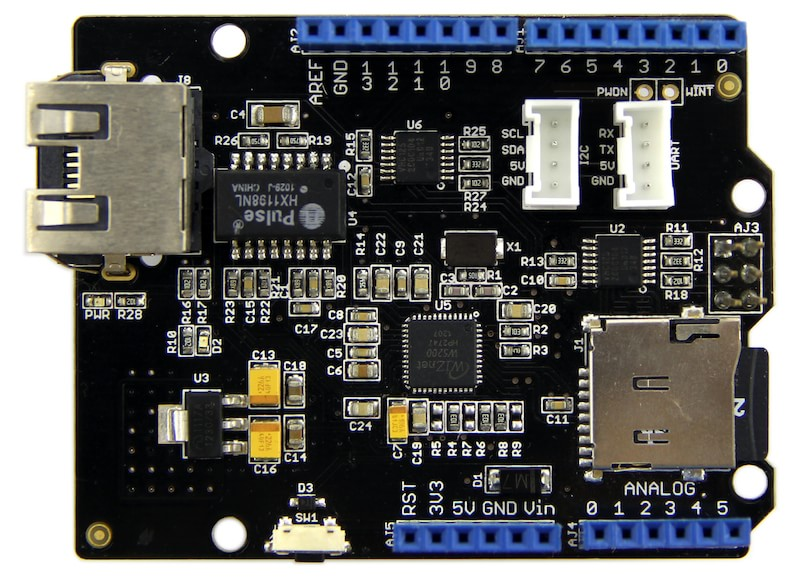
\includegraphics[width=.4\linewidth]{Images/Ethernet_Shield_V2-0}
	\caption{L'Ethernet Shield V2.0}
\end{figure}

Ce \emph{shield} est composé d'une puce W5200 qui permet de lancée des requêtes TCP/UDP sur un réseau Ethernet. Il faut bien évidement le relier à un \emph{switch} ou à une \emph{box} par un câble Ethernet.

\Espace

Pour programmer ce \emph{shield}, il faut aussi utiliser la bibliothéque\footnote{Disponible sur leur dépôt GitHub : \url{https://github.com/Seeed-Studio/Ethernet_Shield_W5200}.} proposée par Seeed Studio.
